\section{Attività Preliminare}
\subsection{Parti compressore}
\begin{figure}[h]
    \centering
    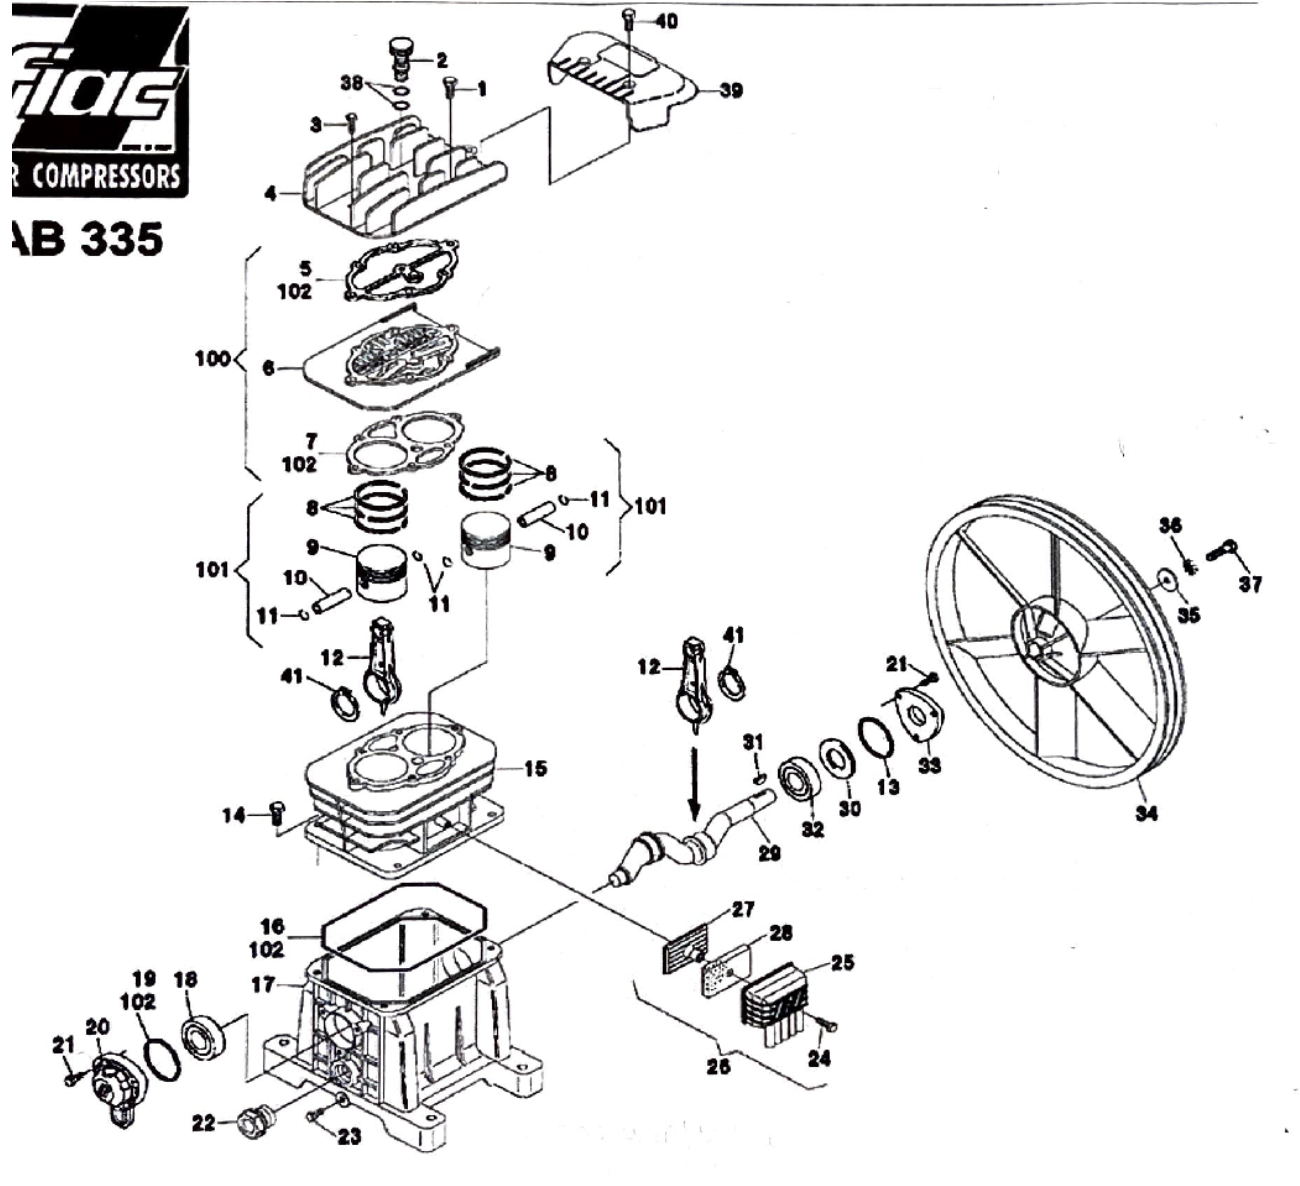
\includegraphics[scale=0.7]{Immagini/EsplosoCompressore.png}
    \caption{Esploso del compressore FIAC AB 335}
        \label{fig:EsplosoCompressore}
\end{figure}
\hspace{-1.3cm}
\begin{tabular}{|l|l|l|l|}
\hline
1&Vite M8x35 UNI-5931&Bullone testata&Acciaio\\
\hline
2&Tappo sfiato&*&*\\
\hline
3&Vite M6x22 UNI-5931&Bullone testa&Acciaio\\
\hline
4&Testata&*&Alluminio fuso\\
\hline
5&Guarnizione&*&*\\
\hline
6&Corpo valvole&Lamelle precaricate&*\\
\hline
7&Guarnizione&*&*\\
\hline
8&Fasce pistone&*&Acciaio\\
\hline
9&Pistone&*&Alluminio fuso\\
\hline
10&Spinotto&D=13 mm&Acciaio\\
\hline
11&Seeger&*&*\\
\hline
12&Biella&*&Alluminio fuso\\
\hline
13&O-Ring&D=53x2 mm&*\\
\hline
14&Vite M8x25 uni-8112&Bullone fissaggio basamento cilindro&*\\
\hline
15&Cilindro&*&Ghisa\\
\hline
16&Guarnizione&*&*\\
\hline
17&Basamento&*&Alluminio\\
\hline
18&Cuscinetto 6203 "17x40x12"&*&*\\
\hline
19&Paraolio&*&*\\
\hline
20&Coperchio&*&Polimerico (AB 245 Plastic)\\
\hline
21&Vite M6x16&Vite fissaggio coperchio&*\\
\hline
22&Indicatore livello olio&AB 245&*\\
\hline
23&Vite M6x16&Vite fissaggio coperchio&*\\
\hline
24&Vite M4x12 UNI-8112&*&*\\
\hline
25&Cassa filtro&*&Polimerico\\
\hline
26&Filtro aspirazione&*&*\\
\hline
27&Flangia supporto filtro&*&*\\
\hline
28&Filtro aspirazione&*&*\\
\hline
29&Albero a gomiti&*&Ghisa sferoidale\\
\hline
30&Distanziale 20x40x7&*&*\\
\hline
31&Linguetta 4x6.5&A mezza luna&*\\
\hline
32&Cuscinetto 6204&*&*\\
\hline
33&Coperchio&*&Polimerico (AB 245 Plastic)\\
\hline
34&Puleggia&$d_{2m}=287\ mm$&Lega di Alluminio\\
\hline
35&Rondella&*&*\\
\hline
36&Rondella anti-svitamento&*&*\\
\hline
37&Vite M8x25 UNI-5739&Vite fissaggio puleggia&*\\
\hline
38&O-Ring 3037&*&*\\
\hline
39&Cover testata&*&*\\
\hline
40&Vite M5x12 UNI-8112&Vite fissaggio cover&*\\
\hline
41&Seeger E 32&*&*\\
\hline
\end{tabular}

\subsection{Componenti, materiali e processi}
\subsubsection{Pistone}
Il pistone è uno degli elementi fondamentali del cinematismo, si muove di moto traslatorio alterno realizzando così la trasformazione del fluido, ed è dotato di sede per spinotto e di gole per fasce elastiche sul mantello.\\
Generalmente le 3 fasce hanno funzioni differenti, ma combinate tra loro:
\begin{enumerate}
    \item \emph{Anello di compressione}: è il più vicino alla sommità del pistone e funge da tenuta per l’aria compressa;
    \item \emph{Raschiaolio a scalino}: è l’anello di mezzo e serve come suggerisce il nome stesso a raschiare via l’olio dalla parete del cilindro nella corsa di aspirazione del pistone, al fine di evitare incrostazioni;
    \item \emph{Raschiaolio a feritoia}: serve a far confluire olio nella parte interna del pistone, in modo da ottenere la lubrificazione dell'accoppiamento spinotto-biella. 
\end{enumerate}
\begin{figure}[h]
    \centering
    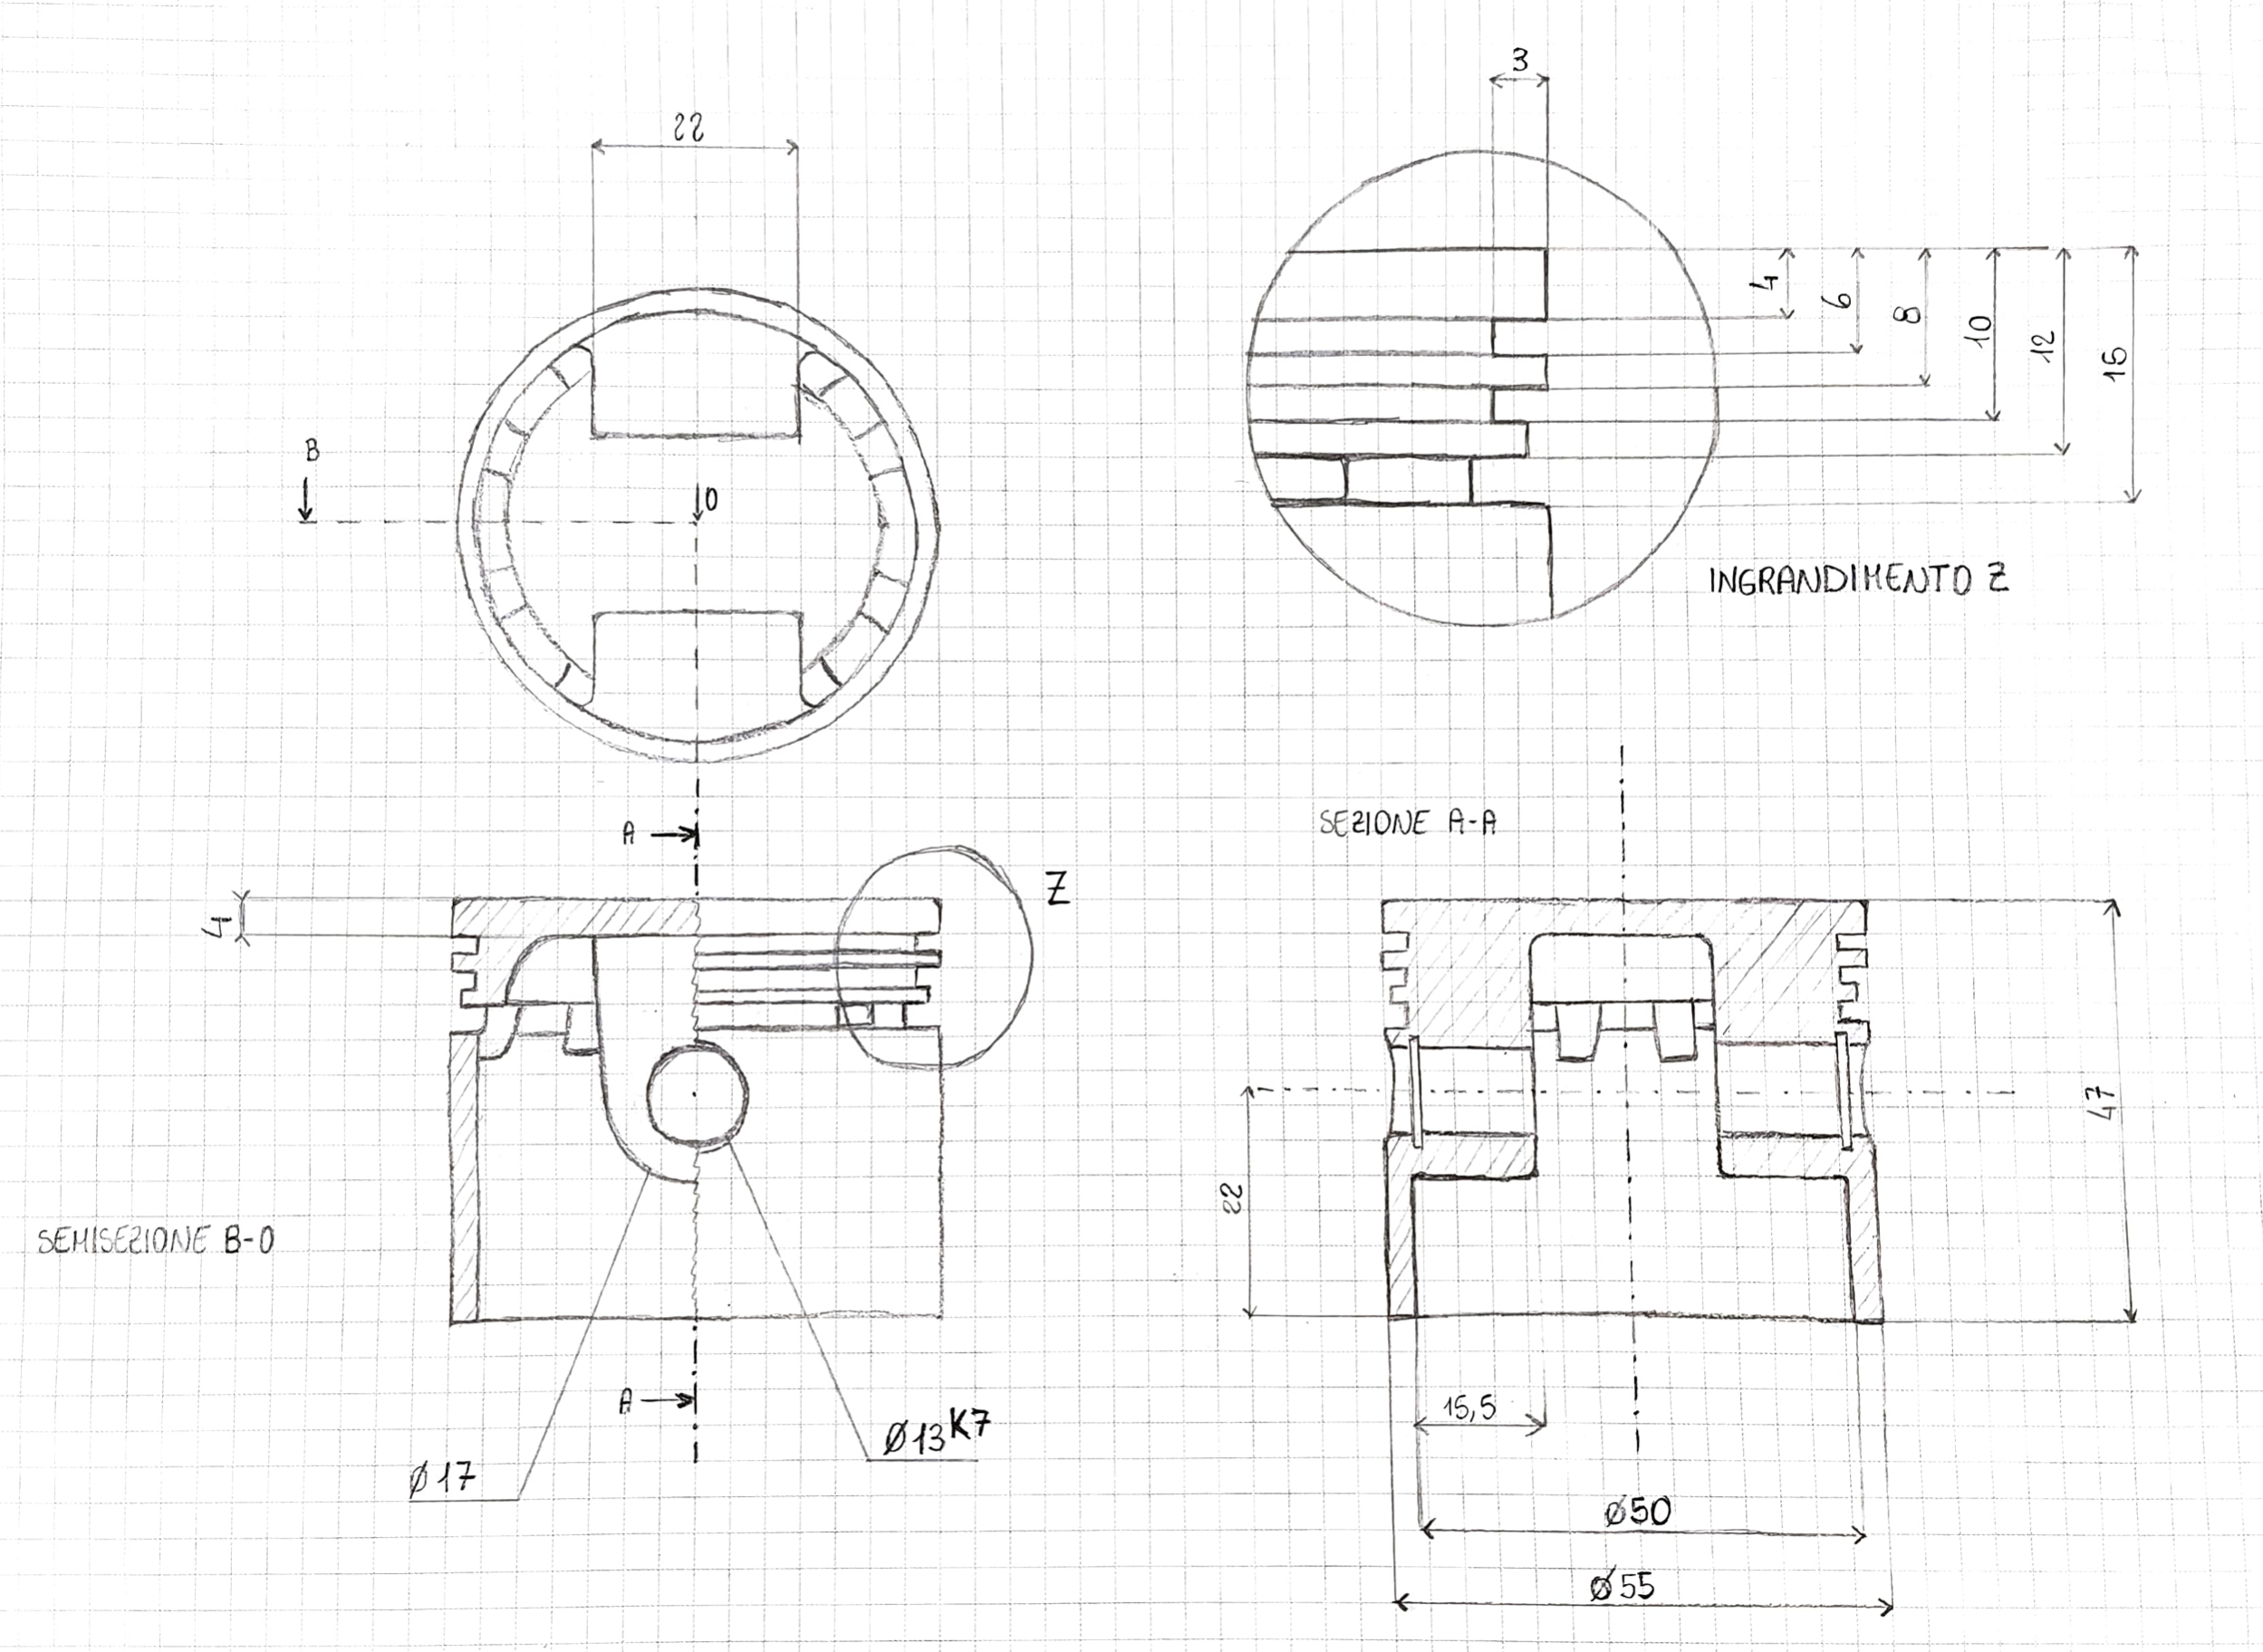
\includegraphics[scale=0.3]{Immagini/SchizzoPistone.png}
    \caption{Disegno a mano libera pistone}
    \label{fig:SchizzoPistone}
\end{figure}
\begin{figure}[h]
    \centering
    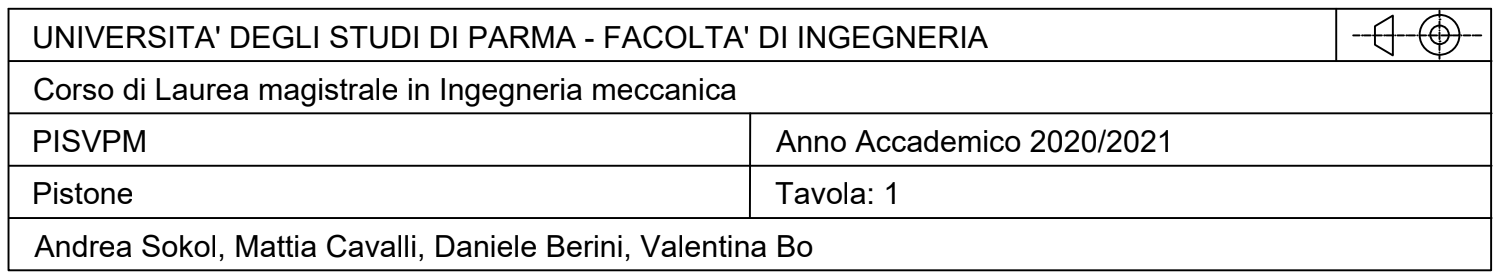
\includegraphics[scale=0.5]{Immagini/CartiglioPistone.png}
    \caption{Cartiglio pistone}
    \label{fig:CartiglioPistone}
\end{figure}
I pistoni nel compressore in esame sono due, con medesimo alesaggio di 55 mm, così come due sono le possibili tecnologie realizzative per tale componente: forgiatura o fusione.\\
La forgiatura è un processo di produzione per deformazione plastica di pezzi metallici, portati ad alta temperatura (superiore a quella di ricristallizzazione) e lavorati poi con ripetuti colpi di una pressa, che cambiano permanentemente la forma del pezzo, senza portarlo a rottura.\\
Si tratta di lavorazioni di stampaggio a caldo dei metalli o leghe metalliche, partendo da un semilavorato portato in condizioni di maggior plasticità.\\
Processo totalmente differente dalla fusione in forme, nel quale il materiale è portato allo stato liquido.\\
\\
Il pezzo considerato sembra essere ottenuto per fusione in conchiglia, vista la spinta cilindricità delle pareti verticali, facilmente ottenibile con quest’ultima lavorazione e meno con la forgiatura. 
Inoltre, la fusione risulta conveniente dal punto di vista economico per una produzione in serie di un elevato numero di componenti.\\
\\
La finitura superficiale esterna indica un’ulteriore lavorazione alle macchine utensili (tornio).\\
\\
Viste le elevate inerzie e l’elevata generazione di calore, dovuta sia al moto dello stantuffo, sia alla trasformazione del fluido, risulta necessario prendere in esame un pistone con caratteristiche di leggerezza e ottima conducibilità termica, in modo da dissipare il calore generato, evitando dilatazioni e mal funzionamenti. \\
\\
La scelta più indicata di materiale ricade quindi su una lega di Alluminio. \\
Tra i materiali utilizzabili per parti lavoranti a caldo con bassa dilatazione (pistoni) ci sono: 
\begin{itemize}
    \item G-AlSi12,7NiMgCu con $R_m$ = 305 Mpa, $R_s$ = 275 Mpa e HB = 125 (riferimento UNI 6250-68)
    \item G-AlCu12 con $R_m$ = 280 Mpa, $R_s$ = 166 Mpa e HB = 120 (riferimento UNI 3040)
\end{itemize}
\subsubsection{Biella}
La biella è un elemento meccanico di collegamento tra albero a gomiti e pistoni, dotato di moto roto-traslatorio.\\
Il collegamento avviene tra la testa di biella e l’albero rotante (lubrificato) da un lato e tra il piede di biella e lo spinotto del pistone dall’altro. \\
\\
La tecnologia realizzativa utilizzata per la biella è lo stampaggio in conchiglia per pressofusione. 
Questo lo si può dedurre dal fatto che in corrispondenza del piano di mezzeria è presente un bordo ad indicare la traccia di apertura dei due stampi. 
Inoltre, sono presenti nervature realizzate per avere uno spessore il più possibile costante dell’oggetto e non avere quindi zone che solidifichino prima di altre, essendo più sottili. 
In ultimo, su una faccia della biella si possono notare i canali di accesso del materiale allo stampo. Questi elementi cilindrici arrivano fino al piano di apertura degli stampi e sono collocati in zone strategiche per aver un flusso di colata omogeneo.\\
\\
Anche in questo caso l’inerzia gioca un ruolo fondamentale per la dinamica del componente. \\
Risulta quindi necessario prendere in esame un materiale con la caratteristica fondamentale di leggerezza. \\
Il materiale con cui è stata realizzata la biella, quindi, è una lega di alluminio per fusione. Tra i materiali utilizzabili si ha:
\begin{itemize}
    \item G-AlSi7MnMg con $R_m$ = 275 MPa, $R_s$ = 195 MPa e HB = 95
    \item Al 2010-T6 con $R_m$ =359 MPa ed $R_s$ = 349 MPa
(riferimento UNI 3599)
\end{itemize}
Gli innesti di silicio, manganese e magnesio servono per aumentare la resistenza meccanica del pezzo.\\
\begin{figure}[h]
    \centering
    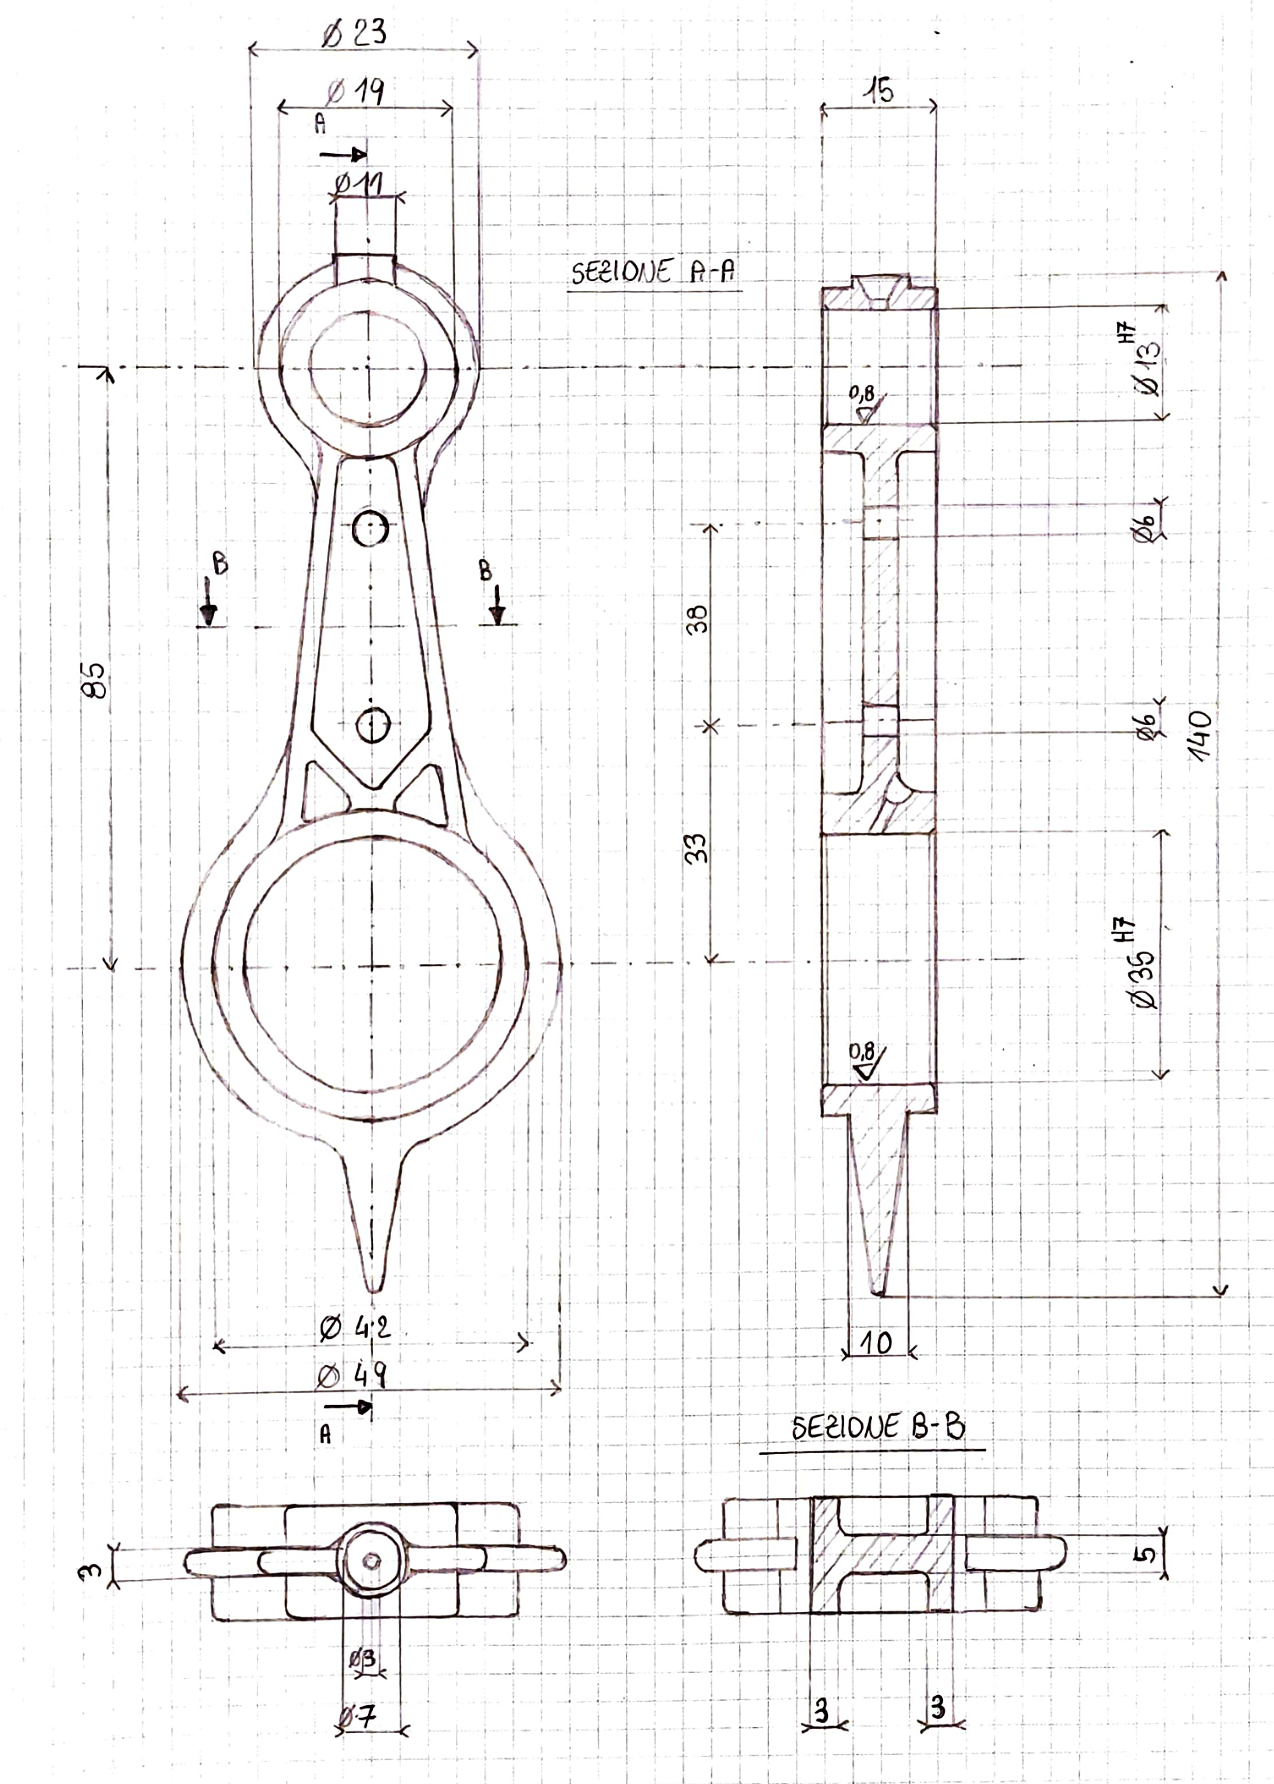
\includegraphics[scale=0.4]{Immagini/SchizzoBiella.png}
    \caption{Disegno a mano libera biella}
    \label{fig:SchizzoBiella}
\end{figure}
\begin{figure}[h!]
    \centering
    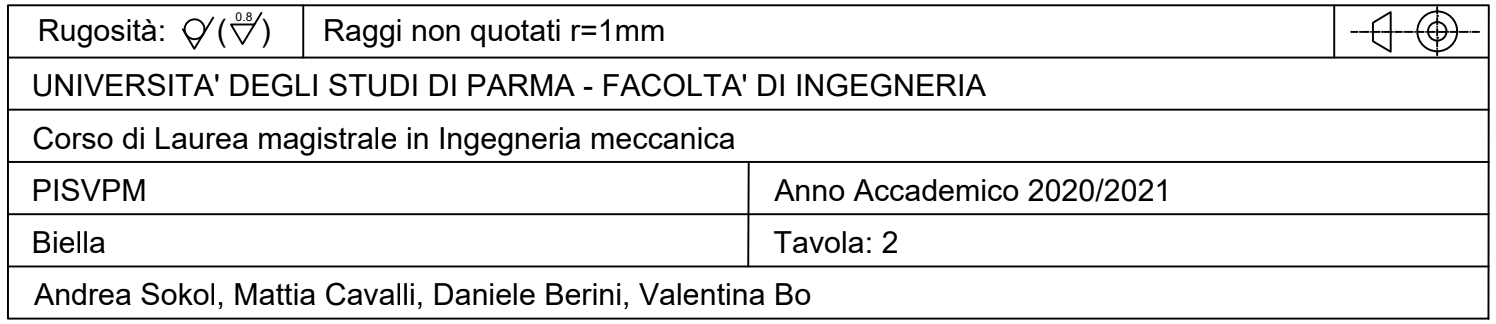
\includegraphics[scale=0.5]{Immagini/CartiglioBiella.png}
    \caption{Cartiglio biella}
    \label{fig:CartiglioBiella}
\end{figure}
\newpage
Dettagli caratteristici:
\begin{itemize}
    \item Si può notare la presenza di una protuberanza longitudinale chiamata “pinna” presente sulla testa di biella, la cui funzione è adibita alla lubrificazione dei componenti, andando a creare una parziale “nebulizzazione” dell’olio presente all’interno del carter. 
    \item Sono presenti canali di lubrificazione appositamente dimensionati per garantire un’ottimale funzionamento delle superfici in moto relativo.
    \item Sono presenti nel fusto di biella due fori realizzati con l’obbiettivo di alleggerire il componente (risparmio quantificabile nell'intorno dei 0,8 g), senza andare a comprometterne la sua resistenza strutturale. 
\end{itemize}
\subsubsection{Spinotto}
Lo spinotto è un elemento di forma cilindrica, che funge da collegamento cinematico tra piede di biella e pistone. All'interno di quest'ultimo sono presenti due sedi per anelli Seeger per vincolare assialmente l'elemento in esame. \\
\\
È un organo che è soggetto a sollecitazioni meccaniche elevate; quindi, deve essere costituito da un materiale resistente all’usura.\\ 
Il processo produttivo vede un tubo trafilato di sezione opportuna, successivamente lavorato al tornio. Per ottenere determinate prestazioni meccaniche, devono essere previste operazioni di indurimento superficiale, il materiale sarà quindi un acciaio, al quale sarà applicato un processo di indurimento diverso a seconda del contenuto di Carbonio. Il componente viene successivamente testato, tramite prove di durezza Vickers, per controllare la buona riuscita realizzativa. In ultimo il pezzo viene rettificato, per riuscire ad avere le caratteristiche di accoppiamento desiderate. \\
\begin{figure}[h]
    \centering
    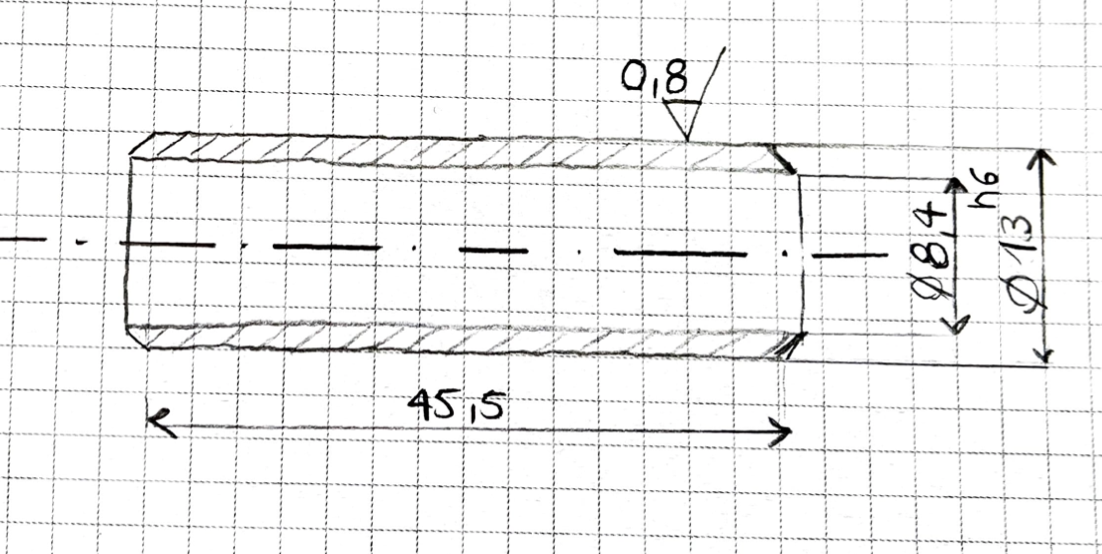
\includegraphics[scale=0.4]{Immagini/SchizzoSpinotto.png}
    \caption{Disegno a mano libera dello spinotto}
    \label{fig:SchizzoSpinotto}
\end{figure}
\begin{figure}[h]
    \centering
    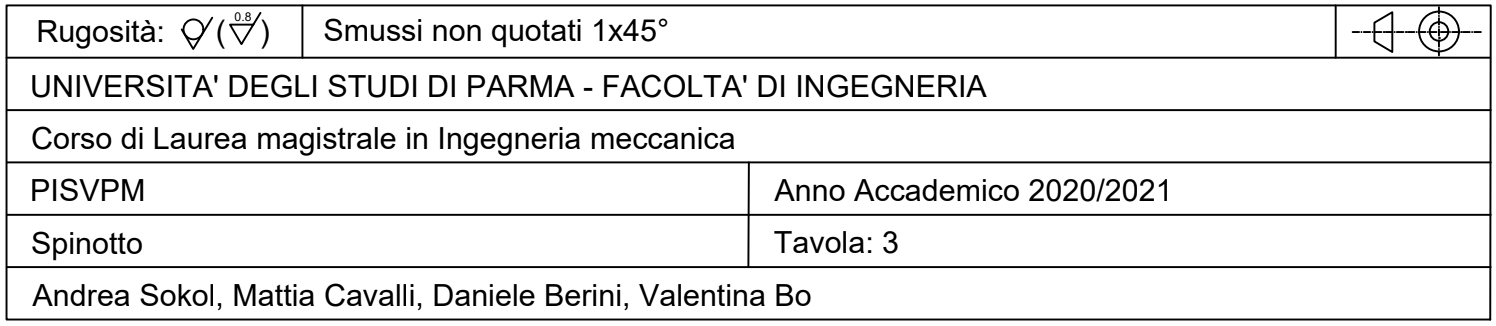
\includegraphics[scale=0.5]{Immagini/CartiglioSpinotto.png}
    \caption{Cartiglio spinotto}
    \label{fig:CartiglioSpinotto}
\end{figure}
\newpage
Tra i materiali utilizzabili si ha:
\begin{itemize}
    \item C15 per cementazione con circa $R_m$ = 620 MPa.
    \item C40 o CrMo12 per nitrurazione con circa $R_m$ = 950 MPa.
    \item C40 o C45 per tempra a induzione con circa $R_m$ = 730 MPa.
\end{itemize}
\subsubsection{Albero a gomiti}
L’albero a gomiti è l’elemento che riceve il moto rotatorio dal motore elettrico e lo trasmette al pistone tramite il cinematismo biella-manovella, convertendolo in moto alternativo. \\
\\
La complessità del pezzo è tale da poterlo ottenere tramite un grezzo di fusione. \\
\\
Le zone adibite all’accoppiamento con la biella presentano diametri maggiorati rispetto al resto dell’albero per ridurre le pressioni di contatto e consentire l’inserimento della biella. \\
Le zone di accoppiamento, il tratto conico e l’altra estremità sono poi successivamente lavorate alle macchine utensili per ottenere la forma definitiva e migliorarne la finitura superficiale. \\
\\
Uno dei materiali più indicati per questo componente è la ghisa. \\
La ghisa è costituita da una matrice (ferritica, perlitica o martensitica) e da particelle di grafite che si possono trovare in forma lamellare o sferoidale. \\
I vantaggi di impiegare questo tipo di materiale sono: 
\begin{itemize}
    \item Economicità (la ghisa avendo più carbonio presenta un punto di fusione più basso, dunque fonderla prevede un minor impiego di energia).
    \item Durezza.
\end{itemize}
Tra le ghise citate quella impiegata per il componente in esame è una ghisa sferoidale, in grado di combinare ai vantaggi prima elencati, prestazioni meccaniche piuttosto elevate ($200\ MPa<R_m<1100\ MPa$).\\
\\
Tra i materiali utilizzabili si ha: 
\begin{itemize}
    \item Gs 350-22 con $R_m$ min. = 350 MPa, $R_s$ min. = 220 MPa e durezza pari minore di 160 HB. Struttura della matrice perlitica-ferritica. (riferimento UNI 4544-74).
    \item Gs 500-7 con $R_m$ min. = 500 MPa, $R_s$ min. = 320 MPa e durezza pari a  168-236 HB. Struttura della matrice perlitica-ferritica. (riferimento UNI 4544-74).
    \item Gs 800-2 con $R_m$ min. = 800 MPa, $R_s$ min. = 480 MPa e durezza pari a  240-335 HB. Struttura della matrice perlitica-ferritica. (riferimento UNI 4544-74).
\end{itemize}
Dettagli caratteristici:
\begin{itemize}
    \item Sono rilevanti le proprietà tribologiche del materiale, ovvero la sua capacità, grazie alla sua finitura porosa, di permettere un miglior insediamento del lubrificante.
    \item La lavorazione delle zone di accoppiamento deve prevedere la realizzazione di uno spallamento per il centraggio della biella durante il montaggio, con apposita gola di scarico. 
    \item Un’estremità presenta un tratto conico con un foro filettato per garantire il fissaggio assiale della puleggia sull’albero a gomiti. È poi presente una sede per linguetta a mezza luna per il trasferimento del moto rotatorio tra i due organi. 
\end{itemize}
\begin{figure}[h]
    \centering
    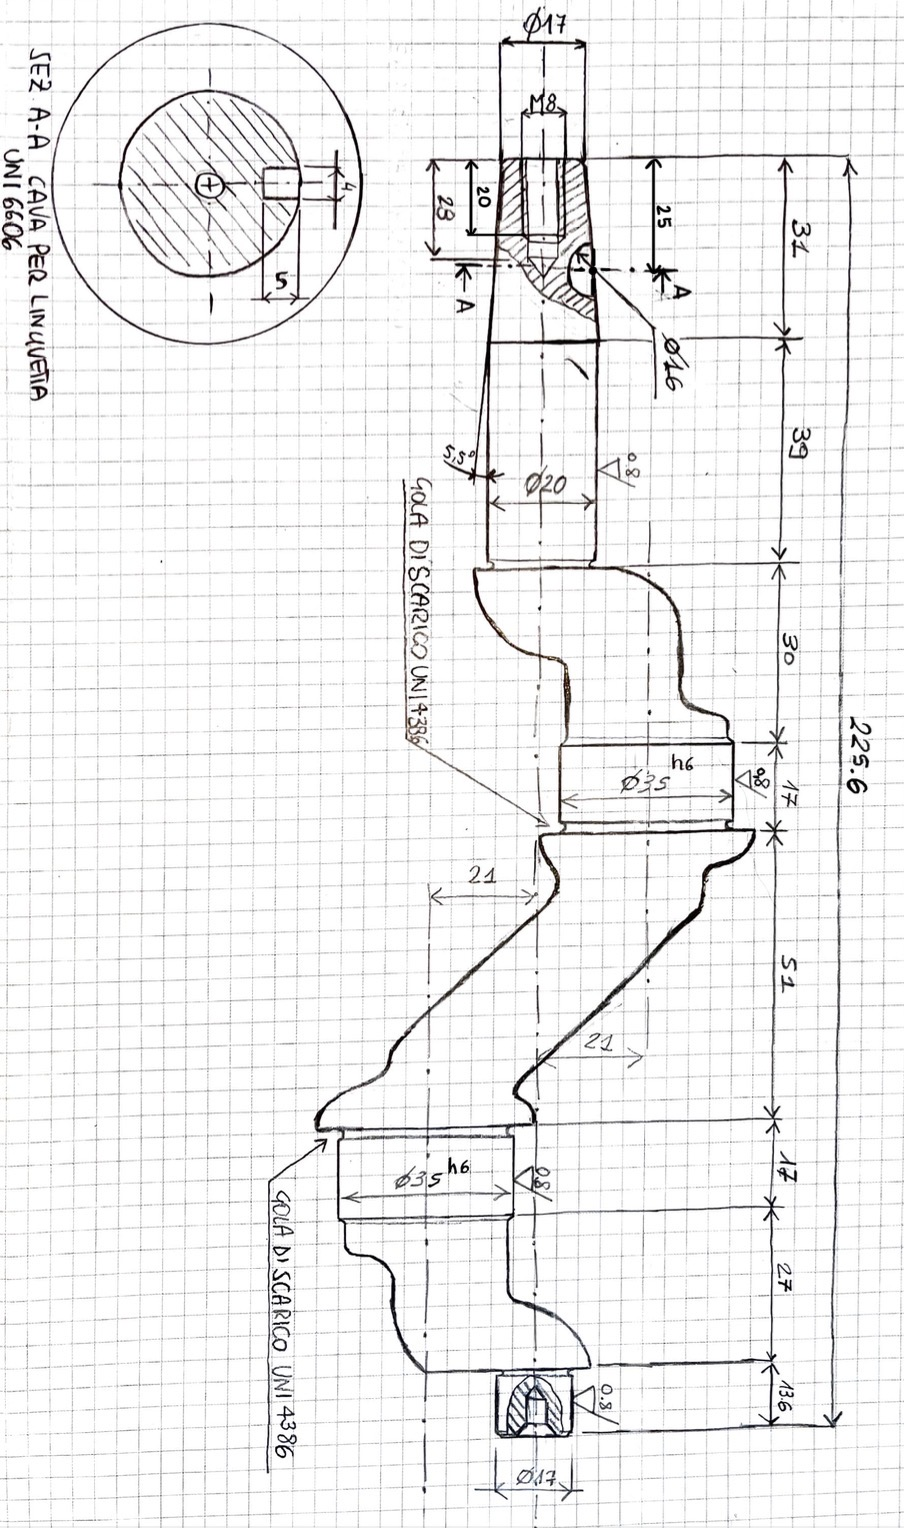
\includegraphics[scale=0.3, angle=90]{Immagini/SchizzoAlbero.jpg}
    \caption{Disegno a mano libera albero a gomiti}
    \label{fig:SchizzoAlbero}
\end{figure}
\begin{figure}[h]
    \centering
    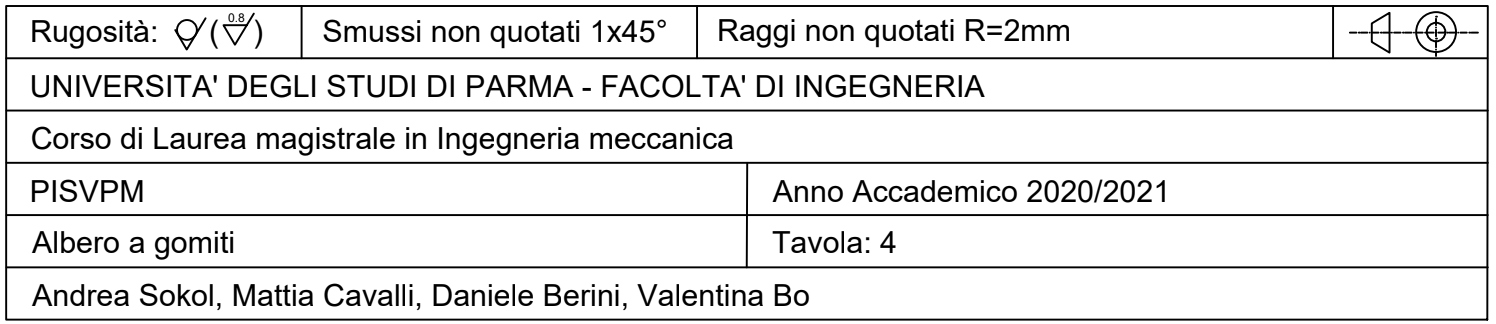
\includegraphics[scale=0.5]{Immagini/CartiglioAlbero.png}
    \caption{Cartiglio albero a gomiti}
    \label{fig:CartiglioAlbero}
\end{figure}
















